\chapter{Maximum flow probleem}
\label{chap:maxFlowProblem}
Om het probleem van het vinden van een maximum flow te kunnen begrijpen, volgt hier een korte introductie in de grafentheorie.

Een graaf is een verzameling punten (knopen) die verbonden zijn door lijnen (kanten). De kanten van een graaf kunnen een richting en/of een gewicht hebben. Een voorbeeld van een simpele graaf is te zien in figuur \ref{fig:6ngraph}.

\begin{figure}[h]
	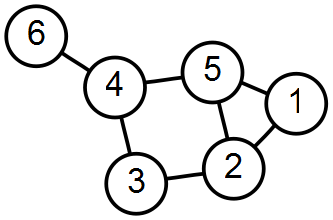
\includegraphics[width=0.5\linewidth]{maxflowproblem/6n-graph}
	\centering
	\caption{Een ongerichte en ongewogen graaf met 6 nodes}
	\label{fig:6ngraph}
\end{figure}

In figuur \ref{fig:flownetwork} is een voorbeeld van een flow network te zien. De flow in deze afbeelding is maximaal, immers de capaciteit van de beide kanten die leiden naar \textit{t} is volledig benut. Tevens te zien dat dit een gerichte (pijlen in plaats van lijnen als kanten) en gewogen (getallen bij de kanten) graaf is.

\begin{figure}[h]
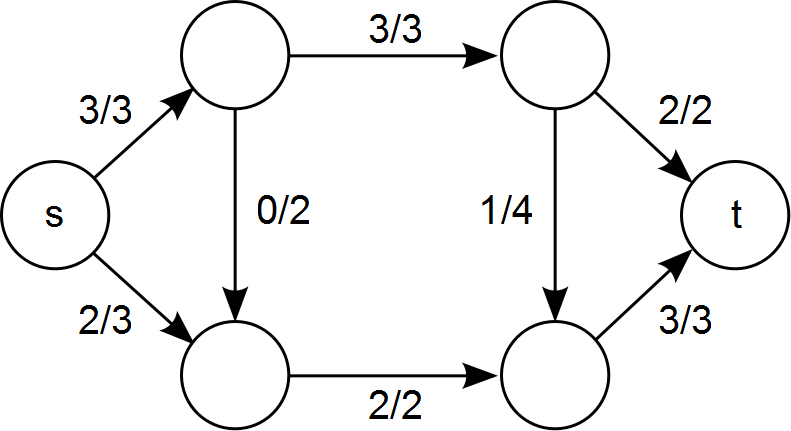
\includegraphics[width=0.5\linewidth]{maxflowproblem/max_flow}%
\centering
\caption{Voorbeeld van een flow netwerk met een maximum flow van \textit{s} naar \textit{t}. De getallen zijn flow / max capaciteit.}%
\label{fig:flownetwork}%
\end{figure}

Het probleem is nu om een flow te vinden van \textit{s} naar \textit{t} die maximaal is. Om dit op te lossen is er het Ford-Fulkerson algoritme, vernoemd naar L.R. Ford en D.R. Fulkerson die dit algoritme publiceerden in 1956. Deze wordt nader toegelicht in paragraaf \ref{sec:fordfulkerson}.

\section{Ford-Fulkerson algoritme}
\label{sec:fordfulkerson}

Het algoritme van Ford \& Fulkerson werkt eigenlijk volgens een heel simpel principe. Zolang er een pad is van \textit{s} naar \textit{t} met beschikbare capaciteit, dan wordt de flow daar langs gestuurd. Dit wordt herhaalt totdat er geen pad meer mogelijk is. Een pad van \textit{s} naar \textit{t} met beschikbare capaciteit wordt een 'augmenting path' genoemd.

De eisen die gesteld worden aan een geldige flow zijn:

\begin{itemize}
	\item De flow mag nooit groter zijn de de capacity van een kant. $0 \leq flow(u,v) \leq capacity(u,v)$
	\item De netto flow van een node is gelijk aan 0. Dit geldt niet voor \textit{s} of \textit{t}.$$\sum_{e \in E^-}\sum_{v \in E^+}{flow(e)-flow(v)} = 0$$
Waar $E^-$ de verzameling van uitgaande kanten is en $E^+$ de verzameling inkomende kanten van knoop $E$ is.
\end{itemize}

Omdat het Ford-Fulkerson algoritme niet aangeeft op welke manier er een 'augmenting path' gevonden dient te worden, zijn er meerdere methodes beschikbaar.
De methodes die onderzocht zullen worden in dit document zijn:

\begin{enumerate}
	\item Depth-first search;
	\item Breadth-first search;
	\item Priority-first search.
\end{enumerate}

\subsection{Pseudocode}

De pseudocode van het Ford-Fulkerson algoritme is te vinden in algoritme \ref{alg:FordFulkerson}.

\begin{algorithm}[h]
\caption{Ford-Fulkerson Algorithm}
\label{alg:FordFulkerson}
\begin{algorithmic}
\REQUIRE Input: Flow network $N$ containing graph $G$
\FORALL{edge $e \in N$}
 \STATE flow($e$) $\gets 0$
\ENDFOR

\STATE $stop \gets$ \FALSE

\REPEAT
\STATE traverse $G$ starting at $s$ to find an augmenting path to $t$ ($\pi$)

\IF{an augmenting path $\pi$ exists}

\STATE $\Delta \gets +\infty$

\FORALL{edge $e \in \pi$}
\IF{ residual capacity($e$) $\leq \Delta$}
\STATE $\Delta \gets $ residual capacity($e$)
\ENDIF
\ENDFOR

\FORALL{edge $e \in \pi$}

\IF{$e$ is a forward edge}
\STATE flow($e$) $\gets $ flow($e$) $+ \Delta$
\ELSE
\STATE flow($e$) $\gets $ flow($e$) $- \Delta$
\ENDIF

\ENDFOR

\ELSE
\STATE $stop \gets$ \TRUE
\ENDIF
\UNTIL{$stop$}

\end{algorithmic}
\end{algorithm}

\section{Analyse}

Voor de analyse van de zoekmethodes worden de grafen uit de figuren \ref{fig:analyseGraaf1} en \ref{fig:analyseGraaf2} gebruikt.
\begin{figure}[h]
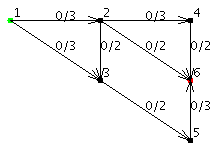
\includegraphics[width=\linewidth]{maxflowproblem/graph1}
\centering
\caption{Analyse graaf 1}
\label{fig:analyseGraaf1}
\end{figure}

\begin{figure}[h]
 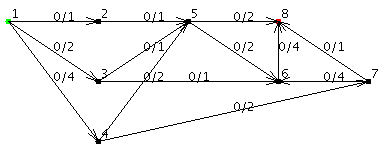
\includegraphics[width=\linewidth]{maxflowproblem/graph2}
\centering
\caption{Analyse graaf 2}
\label{fig:analyseGraaf2}
\end{figure}
